\documentclass[12pt,oneside,brudnopis]{xelatex-mgr/xmgr}

\usepackage{amsmath}
\usepackage{blindtext}

% \defaultfontfeatures{Scale=MatchLowercase}
% \setmainfont[Numbers=OldStyle,Ligatures=TeX]{Minion Pro}
% \setsansfont[Numbers=OldStyle,Ligatures=TeX]{Myriad Pro}
% for fontspec version < 2.0
\setmainfont[Numbers=OldStyle,Mapping=tex-text]{Minion Pro}
\setsansfont[Numbers=OldStyle,Mapping=tex-text]{Myriad Pro}
\setmonofont[Scale=0.75]{Monaco}

\wersja   {wersja wstępna [\ymdtoday]}

\author   {Bartłomiej Kruczyk}
\nralbumu {213603}
\email    {bartlomiej.kruczyk@gmail.com}

\title    {Efektywne algorytmy dla wielokątów wypukłych}
\date     {2014}
\miejsce  {Gdańsk}

\opiekun  {dr Paweł Żyliński}

\newtheorem{problem}{Problem}

\begin{document}

% \begin{abstract}
%   \blindtext[1]
% \end{abstract}

% \keywords{}

% \maketitle

% \introduction

\chapter{Podstawowe pojęcia}
W tym miejscu zostaną przybliżone podstawowe pojęcia związane z
geometrią obliczeniową i problemami dotyczącymi wielokątów wypukłych.

\begin{itemize}
\item{\emph{wielokąt prosty}} --- taki wielokąt, że jedyne punkty
  płaszczyzny należące jednocześnie do dwóch jego krawędzi są jego
  wierzchołkami
\item{\emph{wielokąt wypukły}} --- wielokąt prosty którego wnętrze
  jest zbiorem wypukłym: wszystkie punkty należące do odcinka
  łączącego dwa dowolne punkty ze zbioru wypukłego należą do tego
  zbioru

  \begin{figure}[htp]
    \centering
    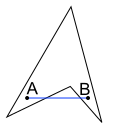
\includegraphics{img/nonconvex}
    \caption{Figura niebędąca wielokątem wypukłym.}
  \end{figure}

\item{\emph{średnica zbioru punktów}} --- średnicą zbioru punktów
  nazywamy największą odległość pomiędzy dwoma punktami należącymi do
  zbioru

\item{\emph{lewoskrętność, prawoskrętność}} --- o kącie mówimy, że
  jest lewoskrętny jeżeli wyznacznik $3 \times 3$ współrzędnych punktów
  $p_1$, $p_2$, $p_3$ kąta jest dodatni, w przeciwnym przypadku
  mówimy, że kąt jest prawoskrętny. Jeżeli $p_i = (x_i, y_i)$ to
  wyznacznik:

  \begin{center}
    \begin{math}
      \begin{vmatrix}
        x_1 & y_1 & 1 \\
        x_2 & y_2 & 1 \\
        x_3 & y_3 & 1
      \end{vmatrix}
    \end{math}
  \end{center}

\item{\emph{proste wspierające}} --- prostymi wspierającymi dla wielokąta
  nazywamy takie proste, które przechodząc przez wierzchołek wielkąta
  nie przecinają jego wnętrza

\item{\emph{punkty antypodyczne}} --- taka para wierzchołków wielokąta przez
  które można poprowandzić równoległe proste wspierające

\item{\emph{notacja wielkiego O}} --- notacja asymptotycznego tempa
  wzrostu wartości funkcji względem jej argumentów, w algorytmice
  stosowana do charakterystyki złożoności obliczeniowej algorytmów
  opisując ilość potrzebnych zasobów (czasu lub pamięci) w stosunku do
  rozmiaru danych wejściowych. Mówimy, że funkcja $f$ jest co najwyżej
  rzędu $g$ (jest ograniczona przez funkcję $g$), gdy istnieją takie
  stałe $n_0 > 0$ oraz $c > 0$, takie że:

  \begin{center}
    $\forall n \geq n_0 : f(n) \leq c \cdot g(n)$
  \end{center}

  \begin{table}[htp]
    \centering
    \caption{Najczęściej wyróżniane rzędy żłożoności obliczeniowej,
      podane według rosnącej złożoności.}
    \begin{tabular}{c c}
      $O(1)$ & stała \\
      \hline
      $O(\log n)$ & logarytmiczna \\
      \hline
      $O(n)$ & liniowa \\
      \hline
      $O(n \log n)$ & liniowo-logarytmiczna \\
      \hline
      $O(n^2)$ & kwadratowa \\
      \hline
      $O(n^c)$ & wielomianowa \\
      \hline
      $O(c^n)$ & wykładnicza \\
      \hline
      $O(n!)$ & ograniczona przez silnię \\
    \end{tabular}
  \end{table}

  W tej pracy efektywnym algorytmem dla wielokąta wypukłego będziemy
  nazywać algorytm o mniejszej złożoności obliczeniowej niż najlepszy
  znany algorytm uogólniony dla wielokąta prostego dla tego samego
  problemu.
\end{itemize}

\chapter{Przegląd problemów}
Przedstawione w niniejszym rozdziale problemy są wspólne dla
wszystkich wielokątów, co pozwala na porównanie rozwiązań i ich
efektywności dla wielokątów prostych i wypukłych. Przy każdym z nich
zostanie przedstawiony problem uogólniony dla wielokątów prostych,
następnie rozwiązanie dla wielokąta wypukłego wraz z analizą
złożoności oraz poprawności algorytmu.

\section{Lokalizacja punktu}
W sytuacji gdy płaszczyznę dzielimy na dwa obszary, z których jeden
jest nieograniczony, drugi natomiast to wielokąt $P$ (na skutek
podziału płaszczyzny na dwie części oraz na podstawie twierdzenia
Jordana o krzywej dla wielokątów wiemy, że $P$ jest prosty) możemy
przedstawić definicję problemu:

\begin{problem}[Lokalizacja punktu]
  Jeśli dany jest wielokąt prosty $P$ i punkt $z$, sprawdzić czy punkt $z$
  należy do wnętrza $P$.
\end{problem}

Problem ten można rozwiązać w czasie $O(n)$ bez przetwarzania
wstępnego. Przypuśćmy, że istnieje prosta pozioma $l$ przechodząca
przez punkt $z$. Musimy teraz rozważyć teraz kilka przypadków:

\begin{itemize}
\item Jeśli $l$ nie przecina $P$ to $z$ leży na zewnątrz wielokąta.
  \begin{figure}[htp]
    \centering
    \caption{(Rysunek) Przypadek 1.}
  \end{figure}
\item W przypadku gdy prosta $l$ przecina $P$ i nie przechodzi przez
  żaden z wierzchołków $P$, jako $p_l$ będziemy oznaczać liczbę
  przecięć $l$ z wielokątem $P$. Wiemy, że lewy koniec $l$ leży na
  zawnątrz $P$, więc przesuwając się po prostej $l$ w prawo w kierunku
  $z$ i przecinając brzeg wielokąta i przechodzimy do jego
  wnętrza. Przy następnym przecięciu z brzegiem $P$ znowu znajdziemy
  się na zewnątrz itd. Widzimy stąd, że $z$ jest zewnętrzny dokładnie
  wtedy gdy $p_l$ jest parzyste.
  \begin{figure}[htp]
    \centering
    \caption{(Rysunek) Przypadek 2.}
  \end{figure}
\item Specjalnym przypadkiem jest ten w którym $l$ przechodzi przez
  jeden lub dwa wierzchołeki. W algorytmie rozważamy przecięcia $l$ z
  krawędziami $P$, więc musimy się zabezpieczyć przed sytuacją w
  której policzylibyśmy przecięcie brzegu $P$ dwukrotnie. Stosujemy tu
  zasadę, że $p_l$ nie zostanie zwiększone dla krawędzi której jeden z
  wierzchołków znajduję się powyżej prostej $l$.
  \begin{figure}[htp]
    \centering
    \caption{(Rysunek) Przypadek 3.}
  \end{figure}
\end{itemize}

Ze względu na to, że każdą krawędź $P$ sprawdzamy tylko raz pod względem
przecięcia z $l$ to mamy do czynienia ze złożonością liniową zależną od
liczby krawędzi wielokąta.

Algorytm dla wielokąta wypukłego wymaga pewnego przetwarzania
wstępnego, ale jest użyteczny w przypadku wykonowyania wielokrotnych
zapytań o przynależność punktu do danego wielokąta. Weźmy punkt $q$
leżący wewnątrz wielokąta wypukłego $P$, może to być np.\ jego środek
wyznaczony przez trzy wierzchołki, a nastąpnie poprowadźmy $N$
półprostych z $q$ przechodzących przez wierzchołki $P$. Płaszczyzna
wraz z wielokątem zostanie podzielona na $N$ części, które nazwiemy
klinami, z których każdy jest podzielony przez krawędź $P$ na dwie
częsci --- jest to wnętrze i zewnętrze wielokąta.

\begin{figure}[htp]
  \centering
  \caption{(Rysunek)}
\end{figure}

Wyszukiwanie położenia danego punktu $z$ składa się z dwóch
etapów. Najpierw określany jest klin w którym leży $z$. Można to
zrobić w czasie $O(\log n)$ używając wyszukiwania binarnego. Punkt $z$
będzie znajdował się pomiędzy promieniami $p_i$ i $p_{i+n}$
podzielonej płaszczyzny wtedy i tylko wtedy gdy kąt $(zqp_i)$ będzie
lewoskrętny, a kąt $(zqp_{i+n})$ prawoskrętny. W następnych krokach
stopniowo zawężamy nasz obszar poszukiwań, do czasu aż odnajdziemy
właściwy klin. Następnie określamy czy $z$ należy do wnętrza lub
zewnętrza znalezionego klinu. Jeśli kąt $(p_{i}p_{i+1}z)$ jest
lewoskętny to $z$ jest wewnętrzny. Określenie skrętności kąta jest
operacją o czasie $O(1)$, więc asymptotyczna złożoność tej części
algorytmu jest logarytmiczna zależna od $N$.

Zastosowane tutaj przeszukiwanie binarne jest możliwe dzięki temu, że
wierzchołki wielokąta wypukłego występują w kolejności kątowej lub
inaczej mówiąc w kolejności krążenia wokół punktu $q$. Przetwarzanie
wstępne dla wielokąta $P$ na które składa się wyznaczenie punktu $q$
oraz umieszczenie wielokąta w strukturze danych wspierającej
wyszukiwanie binarne, może zostać wykonane w czasie $O(n)$.

% \section{Średnica wielokąta}
% \section{Przecięcie wielokątów}
% \subsection{Shamos --- Hoey}
% \subsection{O'Rourke --- Nador}
% \subsection{Separating Axes}
% \section{Zawieranie wielokątów}
% \section{Wyznaczanie prostokąta zawierającego wielokąt}
% \section{Wyznaczanie największej odległości między wielokątami}
% \section{Złączanie wielokątów wypukłych}
% \section{Znajdowanie krytycznych linii wsparcia}
% \section{Oświetlenie wielokąta}

% \summary

% \appendix
% \chapter{Generowanie wielokątów wypukłych o zadanej liczbie
% wierzchołków}

% \bibliographystyle{unsrt}
% \bibliography{xml}

% \listoftables

% \listoffigures

% \oswiadczenie

\end{document}

%%% Local Variables:
%%% coding: utf-8
%%% mode: latex
%%% TeX-master: t
%%% TeX-engine: xetex
%%% End:
